			\documentclass[a4paper,12pt, oneside]{book}
	\usepackage[czech]{babel}
	\usepackage[utf8]{inputenc}

	% Plugin na sloupce
	\usepackage{multicol}

	\usepackage{wrapfig}

	% Plugin na obrazky
	\usepackage{graphicx}

	% Toto je plugin diky kteremu pujde klikat do obsahu
	\usepackage{hyperref}
	\hypersetup{
		colorlinks,
		citecolor=black,
		filecolor=black,
		linkcolor=black,
		urlcolor=black
	}

	% Plugin na hezci nadpis kapitoly
	% https://texblog.org/2012/07/03/fancy-latex-chapter-styles/
	\usepackage[T1]{fontenc}
	\usepackage{titlesec, blindtext, color}
	\definecolor{gray75}{gray}{0.75}
	\newcommand{\hsp}{\hspace{20pt}}
	\titleformat{\chapter}[hang]{\Huge\bfseries}{\thechapter\hsp\textcolor{gray75}{|}\hsp}{0pt}{\Huge\bfseries}


	% Zakladni info o dokumento
	\title{Zálohování a ochrana před ransomwarem}
	\def\topic{Zálohování a ochrana před ransomwarem}
	\def\schoolclass{Oktáva}
	\author{Lukáš Dulík}
	\date{\today} % Tady sa pak moze nastavit jine datum, ted to da vzdycky aktualni


	% Plugin na zahlavi zapati
	\usepackage{fancyhdr}


	\fancyhf{}
	\lhead{\topic}
	\lfoot{Maturitní práce \schoolclass}
	\rfoot{\thepage}

	% Dulezite pro spravne zobrazovani zahlavi zapati
	\pagestyle{empty}
	\fancypagestyle{plain}{}

	\begin{document}

% Zrusi cislovani na zacatecnich strankach
\pagenumbering{gobble}

\begin{titlepage}
    \begin{center}
        \vspace*{1cm}

        \Huge
		Gymnázium Jana Pivečky a Střední odborná škola Slavičín \\

		% Logo GJP
		
\includegraphics[width=0.4\textwidth]{img/gjp.png}

        \textbf{Maturitní práce}

        \vspace{0.5cm}
        \LARGE
        Téma: \topic
    \end{center}

	\vspace{1.5cm}

	% Vyplni zbyvaji prostor
	\vfill

	\vspace{0.8cm}

	\vspace{5pt}
	% Cara nahore
	\hrule
	\vspace{6pt}

	\Large

	\makeatletter
	\begin{multicols}{2}
		\noindent
		Slavičín \\
		Datum: \@date

	\columnbreak
		\noindent
		\null\hfill Třída: \schoolclass \\
		\null\hfill \@author
	\end{multicols}

	\makeatother

	\vspace{5pt}

	% Cara dole
	\hrule

\end{titlepage}

\newpage
\mbox{}
\newpage


\noindent
Prohlašuji, že jsem maturitní práci vypracoval samostatně
a výhradně s použitím citovaných pramenů.

Ve Slavičíně: dne datum jméno, vlastnoruční podpis


\newpage
\section*{Abstrakt}

Cílem této práce je podrobně popsat proces návrhu a realizace nízkonákladového
systému pro zálohování dat.  Výsledný systém má sloužit pro zabezpečení důležitých
dat prostřednictvím pravidelného zálohování.

Základem navrženého zálohovacího systému je jednodeskový počítač Raspberry Pi 5,
ke kterému je pro ukládání záloh připojen pevný disk pomocí USB
dokovací stanice. Pro ochranu a integraci těchto komponent byl navržen a
vytištěn na 3D tiskárně speciální držák. 

Důležitým znakem tohoto provedení byla snaha o využití existujících
hardwarových prostředků. Konkrétně se jednalo o komponenty, které již nebyly
aktivně používány a nacházely se v domácích zásobách.

Tento přístup nejenže snížil finanční náročnost projektu, ale také umožnil
prozkoumat možnosti repurposingu starší technologie pro nové účely.

Realizace byla úspěšná a zálohovací systém se podařilo zprovoznit. Systém
vykazuje rychlosti až 30 MB/s, což je pro vlastní účely adekvátní. Celkově 
se cíl práce podařilo splnit.

\newpage
\section*{Poděkování}

% Udela obsah
\tableofcontents

\clearpage
% Zacatek cislovani stranek
\pagenumbering{arabic}

\chapter{Úvod}

Často opomíjené, ale v počítačových systémech nutné - to je zálohování.
Mnozí z nás uchovávají data na svém vlastním uložišti. Ať už to jsou
fotky z dovolených nebo cenné pracovní dokumenty, mají pro nás vysokou hodnotu
a proto o ně nechceme přijít. Máte vytvořenou zálohu svých dat? 

Lidé jsou zvyklí ukládat své data na USB disky. Ruční zálohování má však své limity,
proto se pojďmě podívat na způsob, jak dělat zálohování poctivě.


\section{Vlastní motivace}

Motivací pro napsání této práce byla nutnost vytvoření zálohy mého
domácího PC. Uchovávám na něm mnoho cenných dat -
jedná se asi o 1 TB fotek a videí. Tyto data mám na HDD, které
slouží již 10 let. Je na konci své životnosti a já nechci přijít o data,
které na něm uchovávám. Proto jsem se rozhodl vytvořit funkční systém 
pro zálohování.

\section{Cíle projektu}

Moje požadavky pro zálohovací systém byly následující. V závěru práce zhodnotíme, 
jestli se podařily splnit.

\begin{enumerate}
	\item Automatizace - Zálohy se vytváří automaticky ve stanovených intervalech
	\item Nízká cena - co nejmenší počáteční i provozní náklady
	\item Spolehlivost - systém nevykazuje chyby
	\item Transparentnost - můžu sledovat průběh zálohování
	\item Error handling - chybové záznamy jdou jednoduše přečíst
\end{enumerate}

\section{Cloud vs On-Premise}

Na trhu je mnoho cloudových řešení pro zálohování. 
Ať už to jsou známé služby jako Google Drive a OneDrive, nebo 
levnější alternativa v podobě Backblaze Backup, cloudové společnosti poskytují 
spolehlivé řešení pro potřeby zálohování. Cena těchto služeb je však vysoká a pro moje účely nevýhodná. 

Kvůli vysoké ceně jsem se rozhodl vytvořit vlastní hardwarové řešení na
zálohování (On-Premise).
Následující kapitoly popisují
proces výběru hardwaru, způsob připojení disku, návrh držáku a softwarovou
konfiguraci systému.


\chapter{Hardware}
\section{Volba platformy}

Před samotnou realizací bylo nutné zvážit různé hardwarové platformy, které by
mohly být pro tento zálohovací systém vhodné. Do úvahy přicházely zejména tři
hlavní kategorie: jednodeskové počítače (konkrétně Raspberry Pi 5), tradiční x86
servery a komerční zařízení pro síťové úložiště dat (NAS). Raspberry Pi 5

\subsection{Raspberry Pi 5}

Jednou z primárních výhod Raspberry Pi 5 pro tento projekt byla jeho dostupnost.
Fakt, že jsem tento jednodeskový počítač již vlastnil a neměl pro něho využití,
znamenal významnou úsporu nákladů, což bylo v souladu s hlavním cílem
práce. Kromě toho se Raspberry Pi 5 vyznačuje nízkou spotřebou energie díky
architektuře ARM. Podle dostupných informací se spotřeba energie Raspberry Pi 5
v klidovém stavu pohybuje mezi 2.2W a 3.4W, přičemž při zátěži dosahuje
přibližně 8.9W až 9.8W . Tato nízká spotřeba přispívá k nižším provozním
nákladům systému v dlouhodobém horizontu, což dále podporuje myšlenku
nízkonákladového řešení.  

\begin{wrapfigure}{r}{0.25\textwidth}
	\centering
	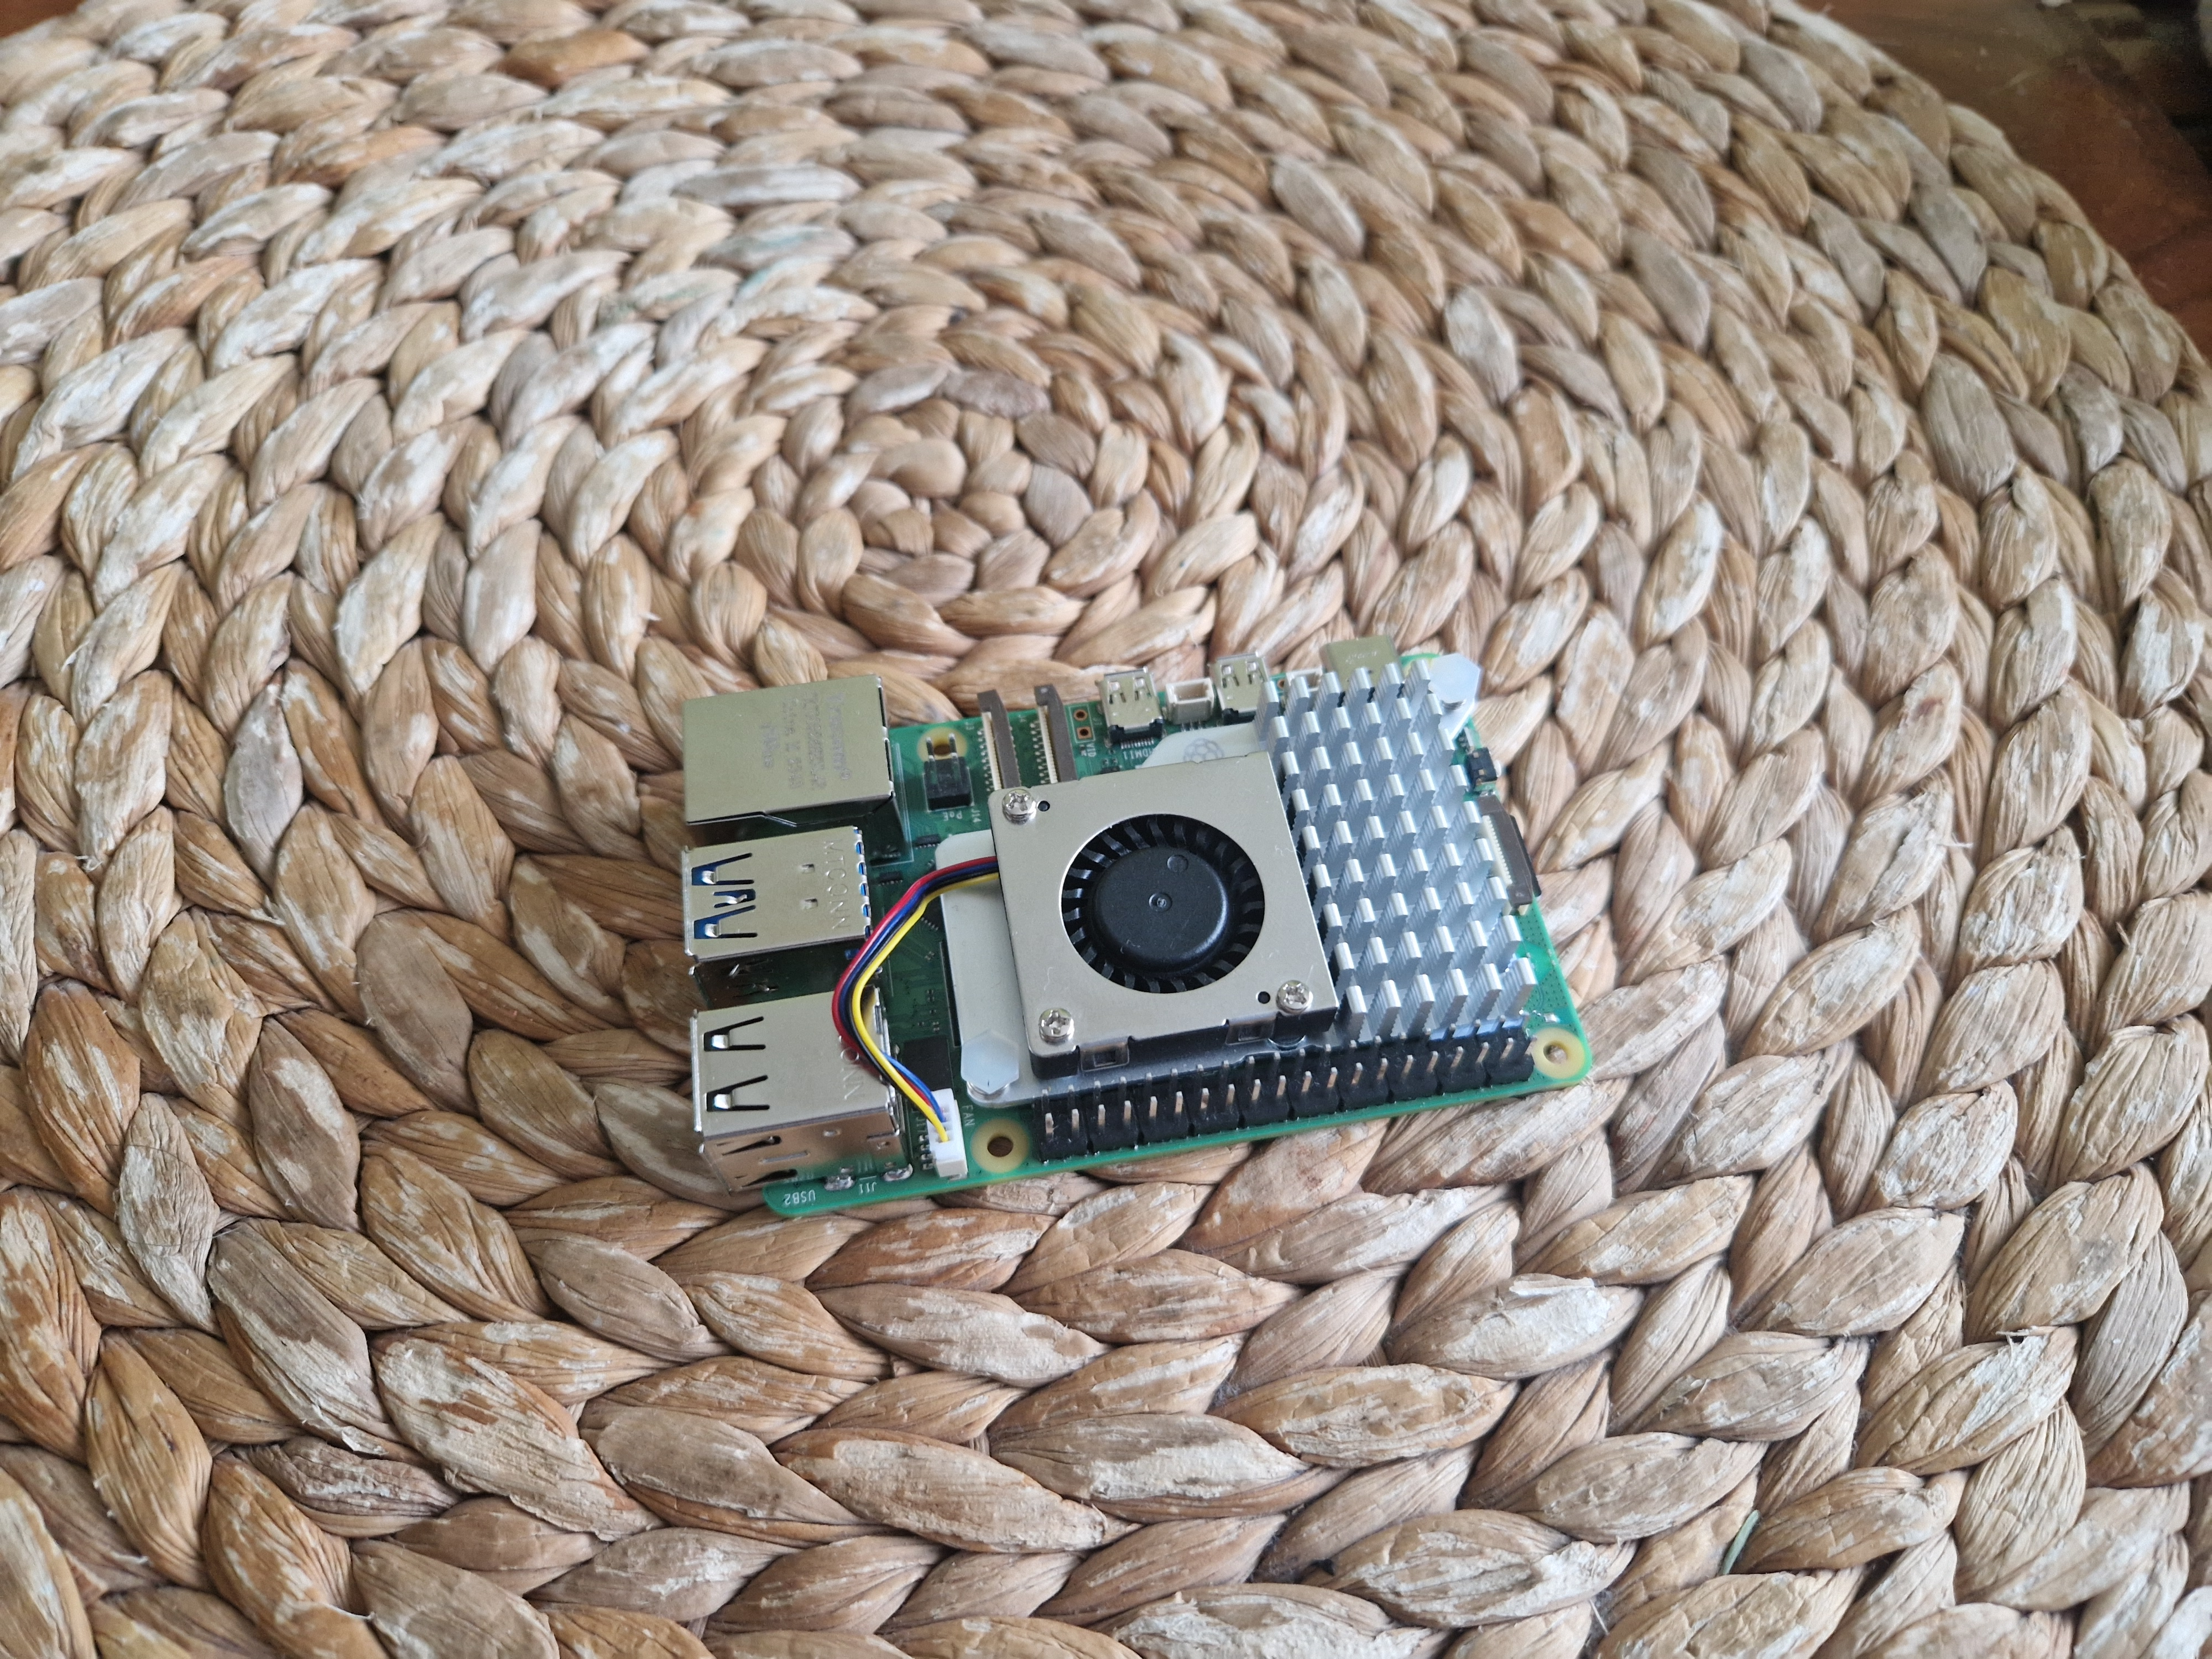
\includegraphics[width=0.25\textwidth]{img/rpi5-active-cooler.jpg}
	\caption{Amazon categories after a search}
\end{wrapfigure}

Na druhou stranu, Raspberry Pi 5 má i své nevýhody. Mezi nejvýznamnější patří
absence nativních SATA portů, které jsou standardním rozhraním pro připojení
pevných disků. Toto omezení vyžadovalo použití alternativních metod pro
připojení úložného zařízení. Dalším aspektem bylo, že samotná deska Raspberry Pi
5 vyžaduje ochranné pouzdro a způsob integrace s připojeným pevným diskem, což
vedlo k potřebě navrhnout a vytisknout vlastní držák. Server x86

\subsection{Server x86}
Tradiční x86 servery nabízejí řadu výhod, které by mohly být pro zálohovací
systém relevantní. Většina serverových základních desek disponuje několika SATA
porty, což umožňuje přímé připojení více pevných disků. Servery jsou také obecně
navrženy pro vysokou spolehlivost a nepřetržitý provoz. Jejich hardwarová
architektura je optimalizována pro serverové úlohy, včetně ukládání dat, a často
nabízejí rozsáhlé možnosti rozšíření, jako jsou další pozice pro disky, PCIe
sloty a větší kapacita paměti RAM. Některé servery podporují i virtualizaci, což
by sice pro jednoduchý zálohovací systém nebylo nutné, ale představuje další
potenciální využití.

Nicméně, x86 servery mají i své nevýhody, zejména v kontextu nízkonákladového
projektu. Jednou z hlavních je vyšší spotřeba energie. Starší x86 servery mohou
v klidovém stavu spotřebovávat odhadem až stovky Wattů , což je výrazně více
než u Raspberry Pi 5. Tato vyšší spotřeba by znamenala vyšší provozní náklady,
což by narušilo cíl nízkonákladového řešení. Dalším faktorem je
pořizovací cena serveru, která i u starších nebo použitých modelů bývá vyšší než
cena jednodeskového počítače, což by překročilo rozpočet studentského projektu.
Navíc, výkon x86 serveru by
pravděpodobně byl pro jednoduchý domácí zálohovací systém zbytečně vysoký.
Komunity jako serverbuilds.net , B24, B25, B26) a r/homeserver)
sice nabízejí návody na stavbu cenově dostupných serverů, ale celkové náklady by
pravděpodobně stále byly vyšší než využití již vlastněného Raspberry Pi.  

\subsection{NAS zařízení}

Komerční NAS zařízení, jako například od společností Synology a QNAP, nabízejí
uživatelsky přívětivé řešení pro síťové ukládání dat. Mezi jejich výhody patří
jednoduchost použití, snadné zapojení a konfigurace. Obvykle obsahují
integrovaný software pro zálohování, sdílení souborů a další funkce .  

Na druhou stranu, NAS zařízení mají i své nevýhody. Často používají proprietární
software, což omezuje možnosti přizpůsobení. Uživatel je také do jisté míry
vázán na ekosystém daného výrobce. Nižší modely mohou mít omezené možnosti
rozšíření. Navíc, použití komerčního NAS zařízení by pro tento projekt znamenalo
menší příležitost k praktickému učení se o konfiguraci hardwaru a softwaru ve
srovnání s vlastním sestavením systému . A co je nejdůležitější, pořizovací cena
komerčního NAS zařízení by byla pravděpodobně vyšší než náklady na komponenty
použité v tomto projektu, což by bylo v rozporu s cílem nízkonákladového řešení.  

\subsection{Závěr}



Na základě výše uvedených úvah jsem se rozhodl jako platformu pro svůj
zálohovací systém použít Raspberry Pi 5. Hlavním důvodem byla jeho dostupnost
, což přímo naplňuje
požadavek na nízké náklady. Dalším významným faktorem byla příležitost k získání
praktických zkušeností s konfigurací hardwaru a softwaru při stavbě vlastního
řešení.


\section{Jak připojit disk k RPI 5?}

Vzhledem k tomu, že Raspberry Pi 5 nedisponuje nativními SATA porty, bylo nutné
zvolit alternativní způsob připojení pevného disku. Pro tento účel jsem zvažoval
dvě možnosti: použití SATA rozšiřujícího modulu (HAT) připojeného přes
PCIe rozhraní, nebo využití USB-to-SATA adaptéru, který může mít formu
dokovací stanice.

\subsection{SATA HAT}
Jedním z dostupných SATA rozšiřujících modulů pro Raspberry Pi 5 je například
Suptronics X1009 PCIe to 5-port SATA HDD Shield . Tento modul se připojuje k
PCIe 2.0 rozhraní Raspberry Pi 5 a umožňuje připojení až pěti SATA 3.0 zařízení.
Podporuje rychlost přenosu dat až 5 Gbps a dokáže napájet jak samotné Raspberry
Pi, tak připojené disky. Je kompatibilní s oficiálním aktivním chladičem pro
Raspberry Pi 5 a podporuje HAT+ STANDBY režim. Důležité je však poznamenat, že
tento modul v současné době nepodporuje bootování z připojených HDD/SSD .

Použití SATA HAT by pravděpodobně zajistilo stabilnější přenos dat a nabídlo
možnost připojení více disků, což by v budoucnu umožnilo implementaci RAID pro
zvýšení spolehlivosti nebo výkonu. Nicméně, pořízení SATA HAT by znamenalo
dodatečný náklad na projekt. Například Geekworm X1009 se prodává za cenu kolem
60 USD. Navíc, pro použití SATA HAT s více disky by bylo nutné navrhnout a
vyrobit vlastní rozsáhlejší pouzdro, které by pojmulo HAT, Raspberry Pi a
všechny připojené disky, s ohledem na napájení a chlazení.  


\subsection{USB-to-SATA adaptér}
Nakonec jsem se rozhodl pro použití USB dokovací stanice AXAGON ADSA-SN, USB 3.2
Gen1 - SATA 6G, 2.5"/3.5" HDD/SSD. Tato dokovací stanice
disponuje rozhraním USB 3.2 Gen1, které nabízí přenosové rychlosti až 5 Gbps,
srovnatelné s SATA 3.0. Je kompatibilní s 2.5" i 3.5" SATA HDD a SSD. Hlavním
důvodem pro tuto volbu byla skutečnost, že jsem tuto dokovací stanici již
vlastnil, což znamenalo nulové dodatečné náklady a plně to
odpovídalo cíli nízkonákladového řešení. Další výhodou je, že USB dokovací
stanice obvykle nevyžadují instalaci speciálních ovladačů,
což zjednodušuje proces nastavení.

Mezi nevýhody patří, že po zapnutí dokovací stanice je připojený disk ve
výchozím stavu vypnutý a je nutné jej ručně aktivovat stisknutím tlačítka. Také
je možné do stanice připojit pouze jeden disk, což omezuje možnosti budoucího
rozšíření a znemožňuje implementaci RAID. Nicméně, pro počáteční cíl vytvoření
jednoduchého zálohovacího systému s jedním diskem představuje tato USB dokovací
stanice funkční a nákladově nejefektivnější řešení.

\section{Návrh držáku na RPI}

Jedním z požadavků projektu bylo fyzické propojení Raspberry Pi 5 a USB dokovací
stanice do jednoho celku. K tomuto účelu bylo nutné navrhnout speciální držák.
Dalším důležitým aspektem byla ochrana samotného Raspberry Pi 5 před mechanickým
poškozením a zkraty, což vyžadovalo umístění desky do nějakého pouzdra.

\begin{figure}[h]
\caption{Example of a parametric plot ($\sin (x), \cos(x), x$)}
\centering
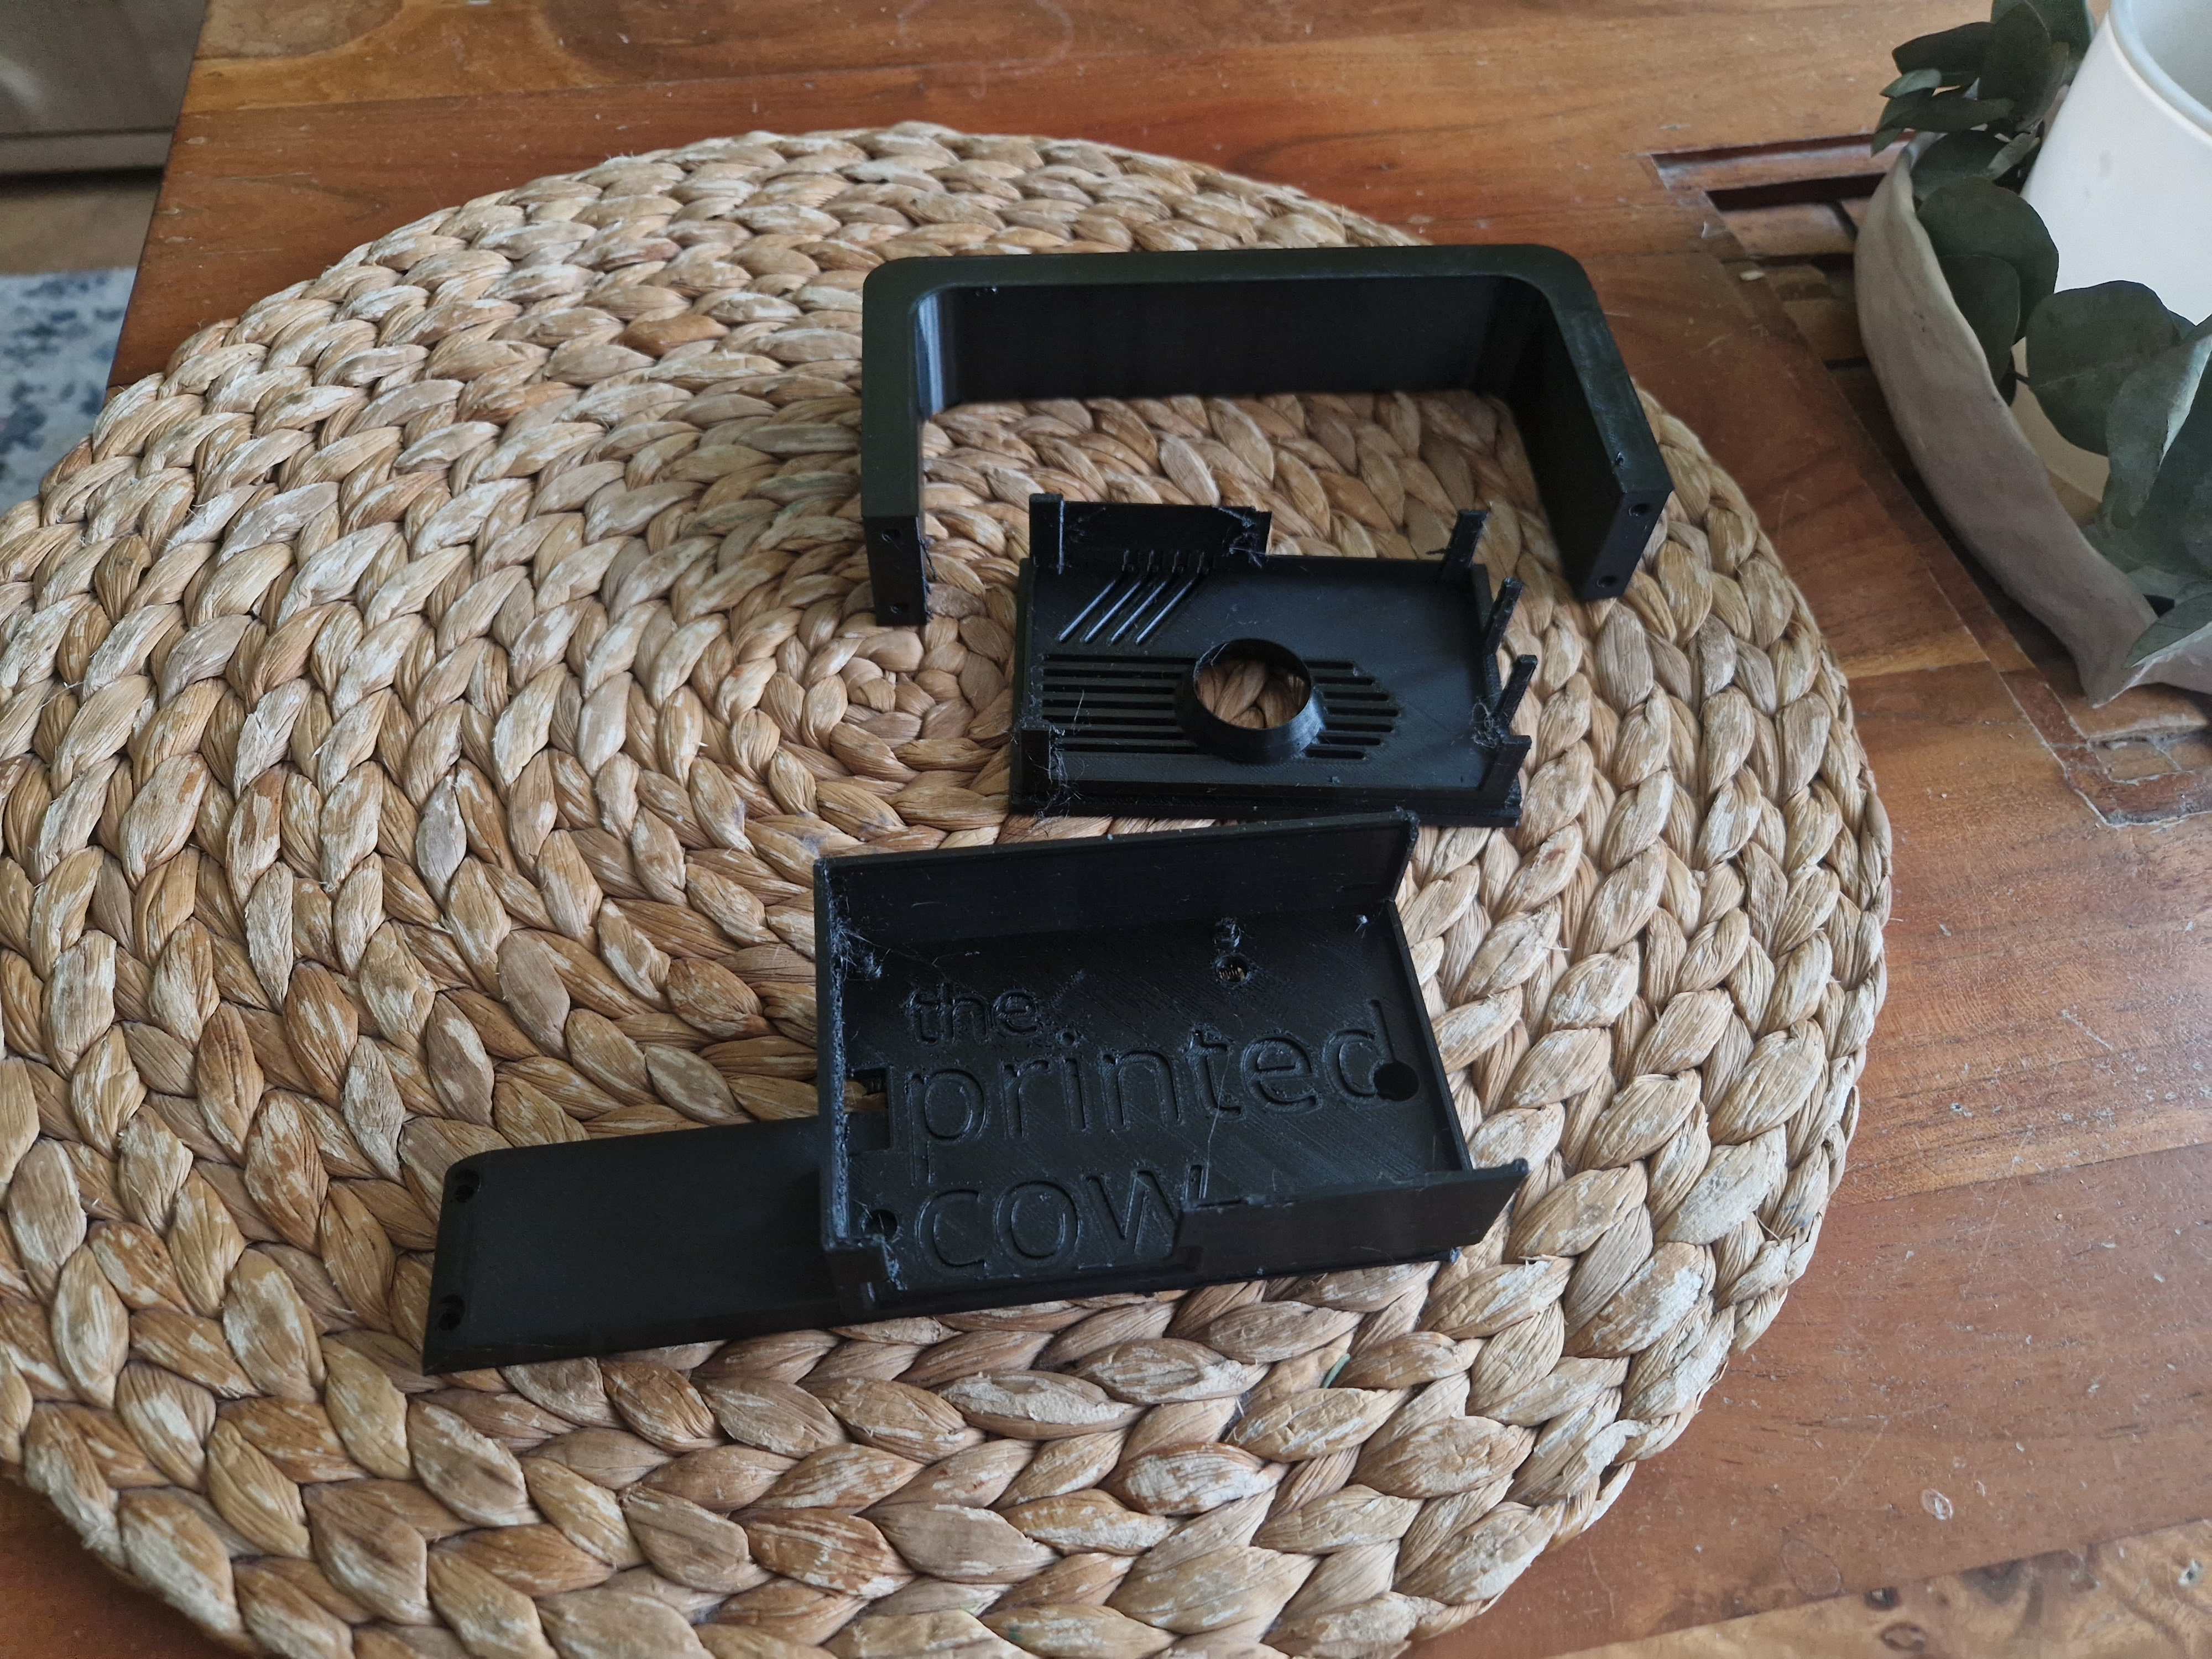
\includegraphics[width=0.5\textwidth]{img/dily-zvlast.jpg}
\end{figure}

Pro návrh držáku jsem použil program Autodesk Fusion 360. V tomto softwaru jsem
vytvořil objímku, která je navržena tak, aby pevně držela USB dokovací stanici.
Tuto vlastní navrženou objímku jsem následně spojil s existujícím krytem pro
Raspberry Pi 5, který jsem stáhnul z internetu. 

\begin{figure}[h]
\caption{Example of a parametric plot ($\sin (x), \cos(x), x$)}
\centering
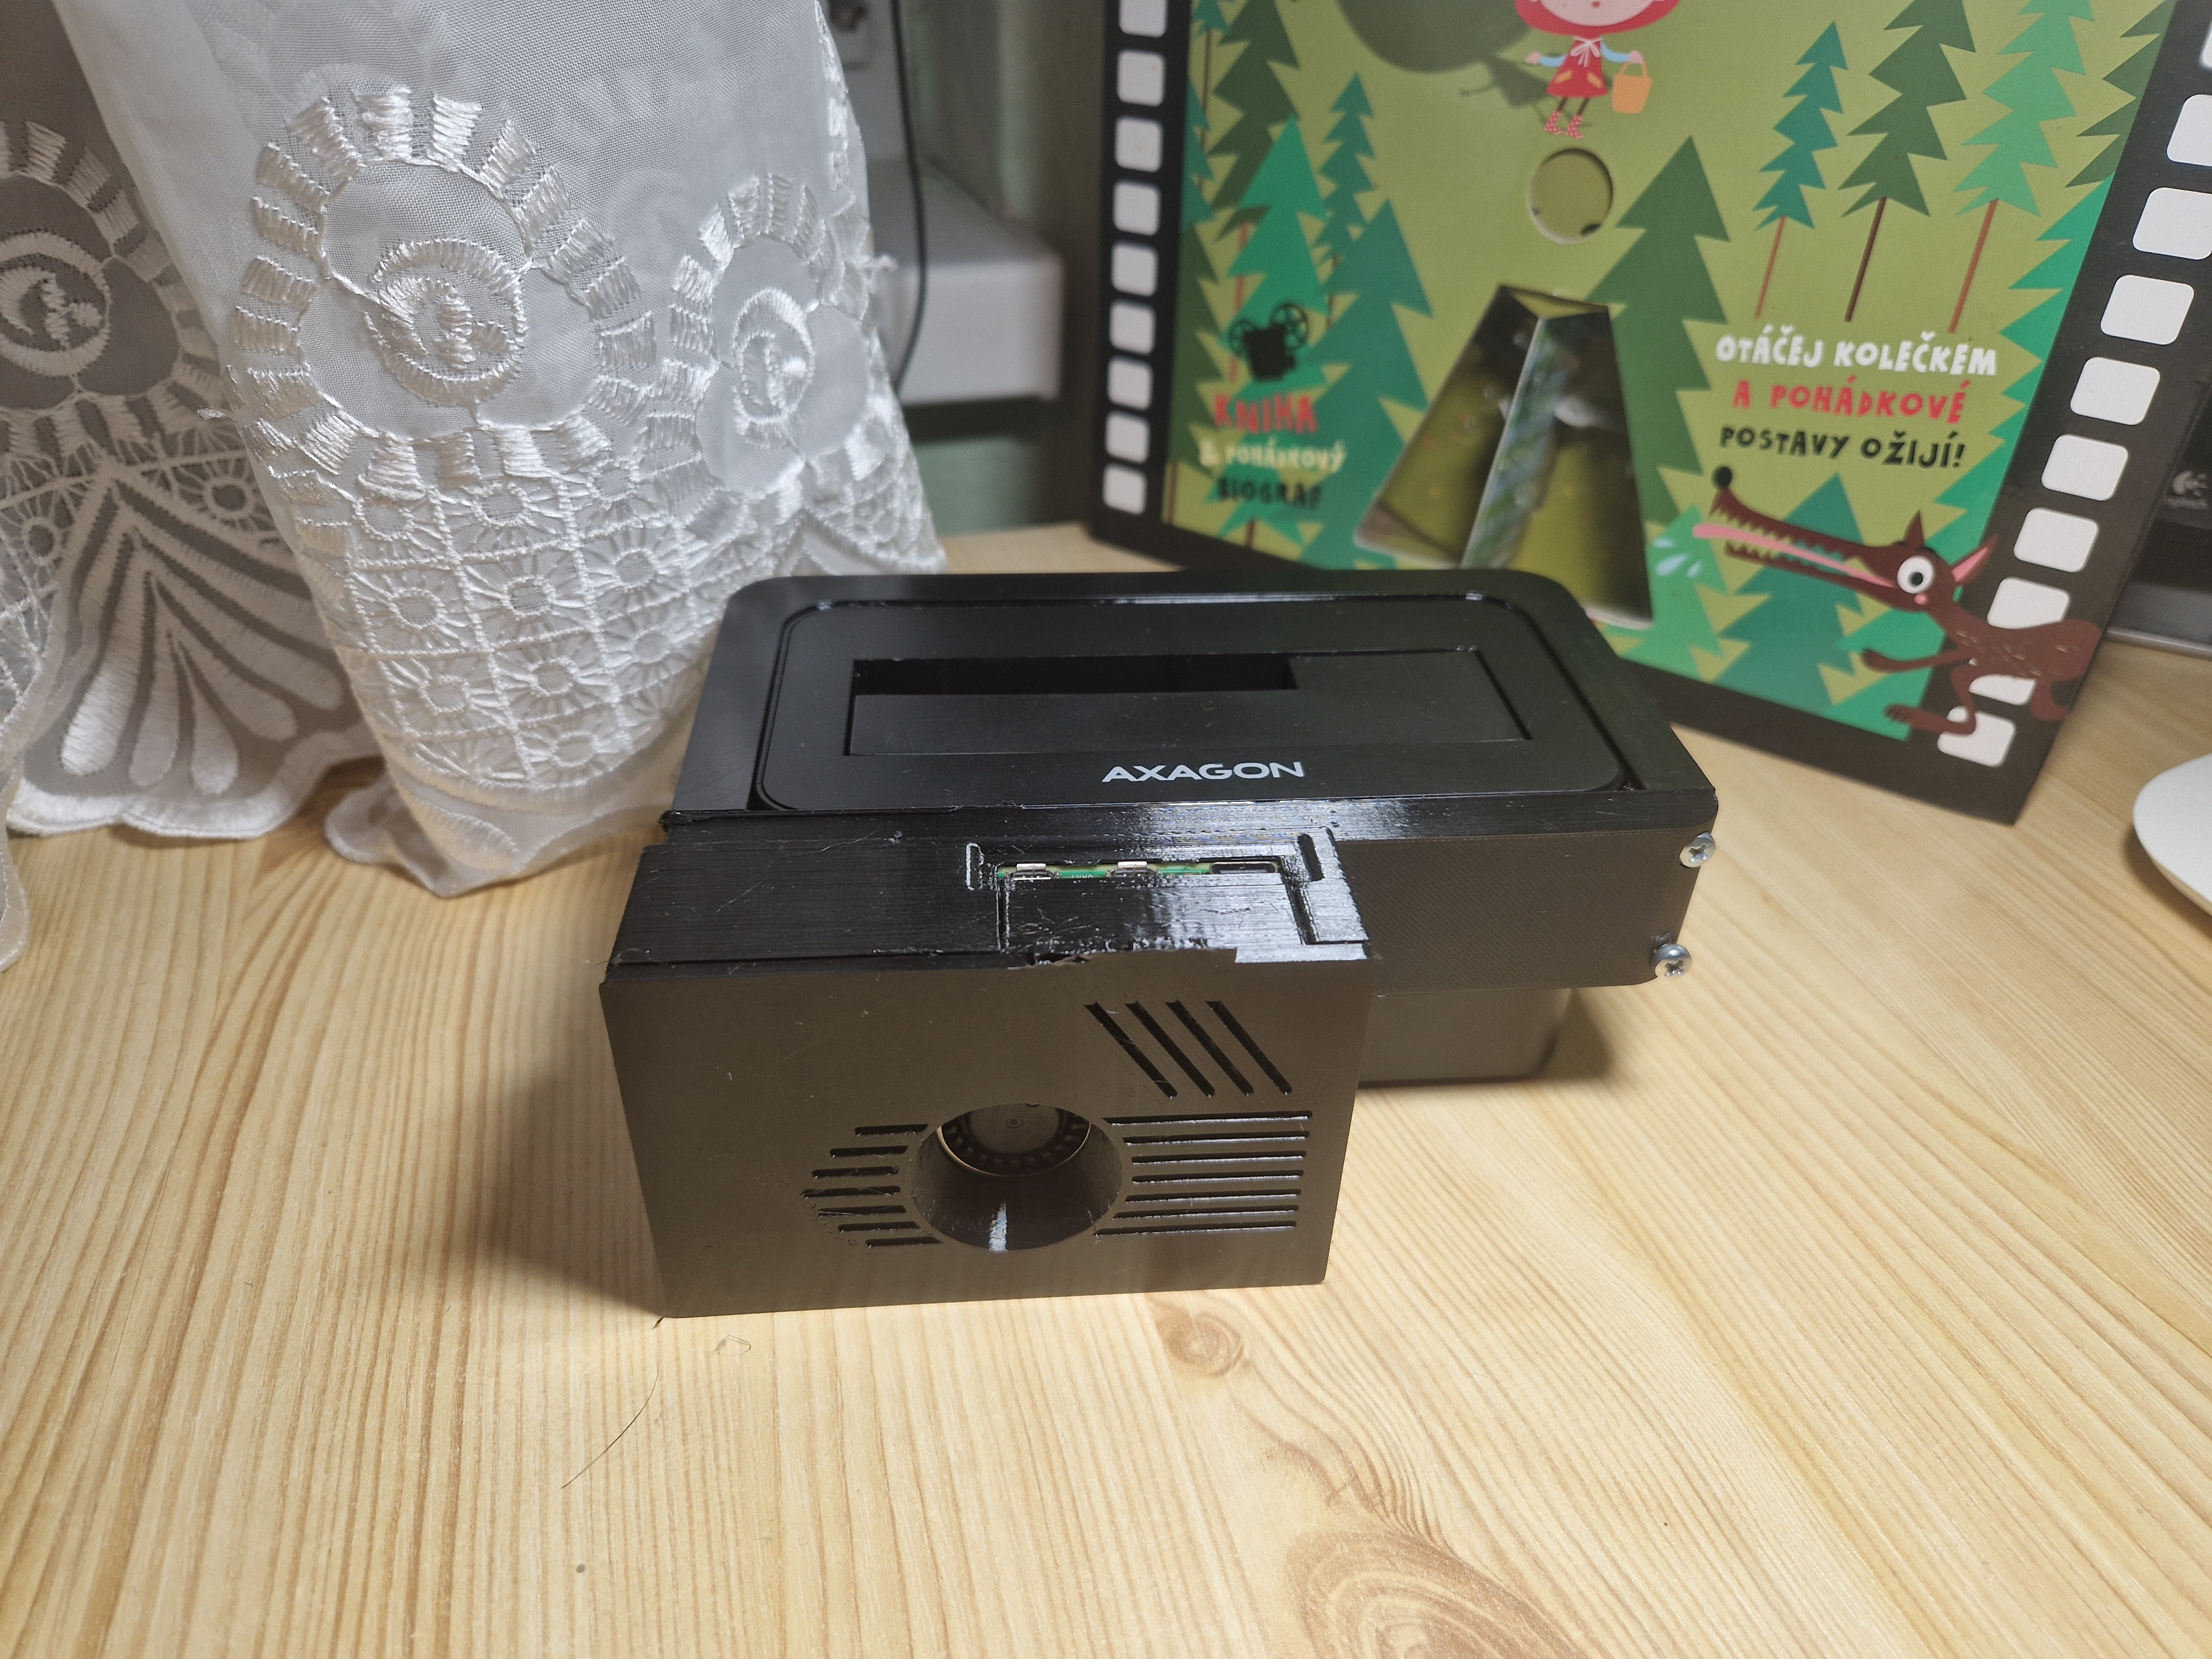
\includegraphics[width=0.9\textwidth]{img/skladani4.jpg}
\end{figure}

Použití hotového krytu pro Raspberry Pi mělo tu výhodu, že již zajišťoval
základní ochranu desky a měl esteticky přijatelný vzhled. Nevýhodou tohoto
řešení je však správa kabelů. Propojení Raspberry Pi, dokovací stanice a jejich
napájecích kabelů vyžaduje pečlivé uspořádání, aby nedocházelo k nepořádku a
potenciálním problémům s konektivitou . 

I přes tuto výzvu s kabelovým managementem, kombinace vlastního
držáku pro dokovací stanici a staženého krytu pro Raspberry Pi poskytla funkční
a vizuálně uspokojivé řešení pro integraci hardwaru.

% TODO: kabely

\chapter{Software}

Pro správu zálohovacího procesu bylo nezbytné vybrat vhodný zálohovací software.
V úvahu přicházelo několik open-source řešení, která jsou kompatibilní s
Raspberry Pi, jako například rsync, borgbackup nebo kopia.

Nakonec jsem se rozhodl pro použití softwaru Kopia. Kopia je moderní open-source
nástroj pro zálohování, který nabízí funkce jako šifrování, deduplikace,
komprese a podporu různých úložišť. Instalace Kopia na domácím PC je poměrně jednoduchá, na Linuxových 
distribucích jde stáhnout prostřednictvím správce balíčků.

Pro vytvoření Kopia repozitáře jsem použil grafické rozhraní Kopia UI.
Následně jsem nakonfiguroval zálohovací politiky, které
definují, jaká data se mají zálohovat, jak často a kolik verzí se má uchovávat.

Kopia běží na domácím PC a data ukládá na Raspberry Pi pomocí protokolu SFTP.
Raspberry Pi tak plní funkci NASu a neběží na něm žádný zálohovací software.

Výběr programu Kopia umožnil vytvořit robustní a funkcemi bohaté zálohovací
řešení, které nabízí pokročilé funkce pro zajištění integrity a efektivity
zálohování.  










\chapter{Závěr}


\chapter{Seznam použité literatury}

\chapter{Seznam odkazů}



\chapter{Seznam obrázků}
\listoffigures


\chapter{Seznam příloh}


\end{document}

